\documentclass[12pt]{article}
\usepackage[utf8]{inputenc}
\usepackage{amsmath}
\usepackage{amssymb}
\usepackage{graphics}
\usepackage{graphicx}
\usepackage{array}
\usepackage{hyperref}
\usepackage{xcolor}
\usepackage{float}
\usepackage[french]{babel}
\usepackage[T1]{fontenc}
\usepackage[a4paper, total={6.5in, 10in}]{geometry}

\begin{document}
\begin{titlepage}
	\centering
	
	
	\vspace{0.5cm}
	{\Large \scshape\bfseries KT IT responsible}
	\vspace{0.5cm}

	{ \Huge }
	

	{\itshape V2023.1 \large  Jacques HOGGE \par}
	{\itshape V2023.2 \large  Jacques HOGGE \par}

	\vspace{5cm}
	
	
	\textit{Il s'agit d'une reformulation du KT d'avant car on a du changer de site et donc tous n'est plus trop a jour}
	

	\vfill
	
    {\Large  \today}
\end{titlepage}
\newpage

\section{Wordpress}\label{Wordpress}
	Notre site est gerer par Wordpress\footnote{oui c'est null mais accessible a tous le monde} et héberger sous OVH. Il faudra donc un compte Wordpresssur chaque site (adresse perso ou BEST comme vous voulez). Pour avoir les access au site il faut voire \autoref{}
	
	\subsection{Mises a jours}
		Il faut faire attention de bien garder Wordpress a jour avec tous les extension(Elementor, Theme, W3,\dots). Des mises a jour qui traine peuvent amener a des problème visuel sur le site et/ou des problème de sécurité et nous n'avons pas envie de refaire encore une fois un nouveau site, de plus sela amène un peu de fraicheur au site. Pour mettre a jour, c'est facile, il suffit d'accéder au menu a gauche dans le tableau de bord $\rightarrow$ Mise a jours. Parfois il y a des petite bulles rouges qui indique que une mise a jours est présente.
		\begin{figure}[htp]
			\centering
			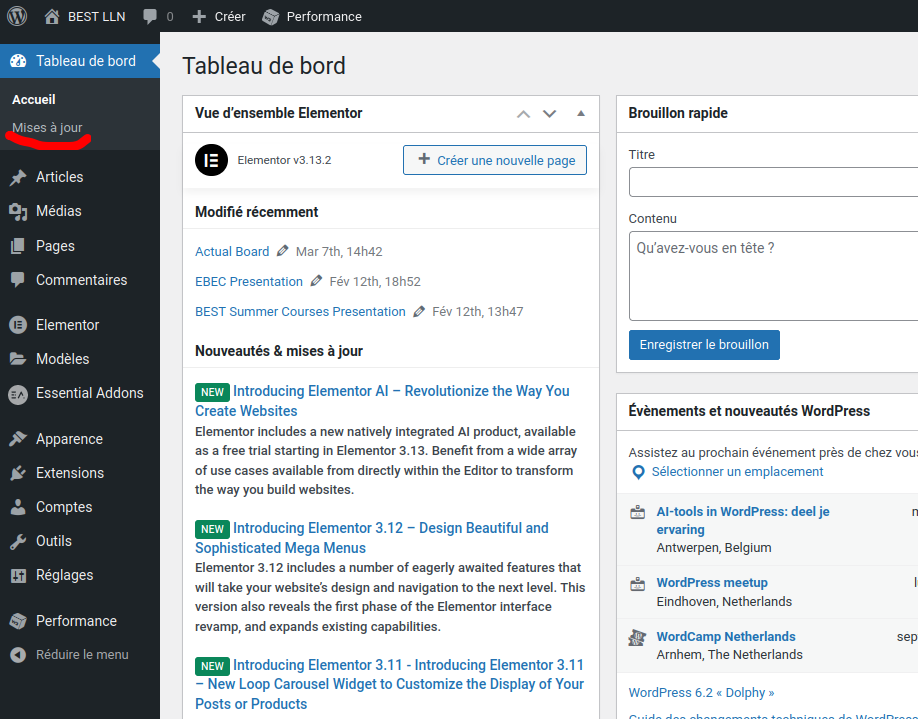
\includegraphics[width=0.6\textwidth]{img/MiseAJours.png}
		\end{figure}
		
	 	 Il existe plusieurs types de mise a jours.
	 	 \begin{itemize}
	 	 	\item MAJ extensions
	 	 	\item MAJ themes
	 	 	\item MAJ Wordpress
	 	 \end{itemize}
	 	 
	 	 \textcolor{red}{Attention pour les MAJ Wordpress, toujours faire une sauvegarde du site avant. Je vous conseille meme de le faire pour n'importe quelle MAJ on est jamais trop prudent.}
	 	 
	 	 Il arrive parfois que faire toutes les MAJ ensemble d'un coup amène a des problème. Il est parfois judicieux de les faire une a la fois.
	 	 
	 	 Si jamais tu vois que le site est cassé apres la mise a jour, pas de PANIQUE. Soit c'est minime et tu sais le modifer toi meme sur Wordpress. Ou alors tu peux aller sur OVH pour restaurer un ancienne sauvegarde du site (cf \autoref{}). Attention de choisir une sauvegarde assez récente.
	 	 
	 \subsection{Évènements}
	 	Il faudra a certain moment crée une nouvelle page afin de parler d'un évènement que l'on organise (EBEC, Hackathon, Summer ...). Normalement c'est les MO (ou responsable du poste) de l'event qui est responsable de rédiger l'article a mettre sur la page.Il faut donc pas hésiter a les SPAM comme des porc afin d'avoir l'article a temps. Je vous conseille de poser un DL sinon il ne va jamais vous faire ton article car il est "occupé a autre chose".
	 	
	 	Bien que il y a Facebook, Insta, Onlyfans pour faire la pub de nos events et que le site est un peu obsolète, celui-ci sert principalement d'archive de CECI-BEST. Il faut cependant quand meme faire l'article car celui-ci permet un visuel pour nos sponsos.
	 	
	 	Pour faire une page, il suffit de copier une page déja faite et changer le titre, les photos, le texte, les responsable et ajouter des boutons qui ramène vers le formulaire d'inscription et/ou a l'event Facebook.
	 	 
	 \subsection{Créer une page}
	 	Rien de tres sorcier, il suffit d'aller sur le tableau de bord de Wordpresse $\Rightarrow$ Pages $\Rightarrow$ Ajouter
	 	\begin{figure}[htp]
			\centering
			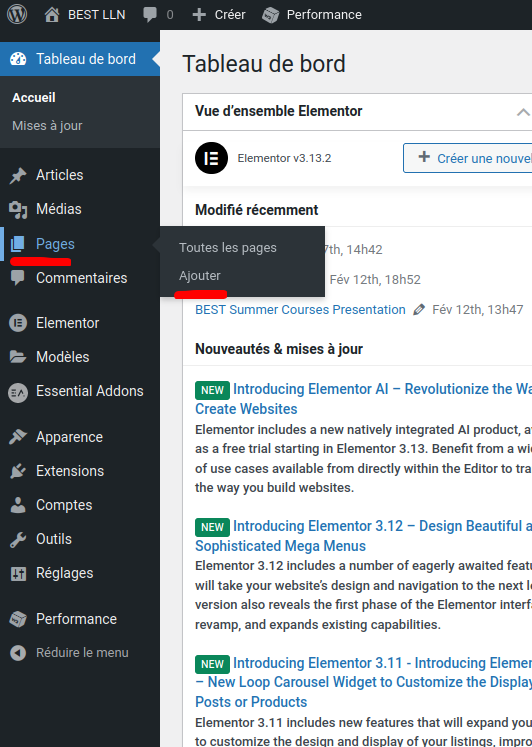
\includegraphics[width=0.6\textwidth]{img/CreerPage.png}
		\end{figure}
		
		Il suffit ensuite d'editer le perma lien afin qu'il soit asser jolie. Pour cela : Colonne de droite $\rightarrow$ Page $\rightarrow$ URL
		
		\begin{figure}[htp]
			\centering
			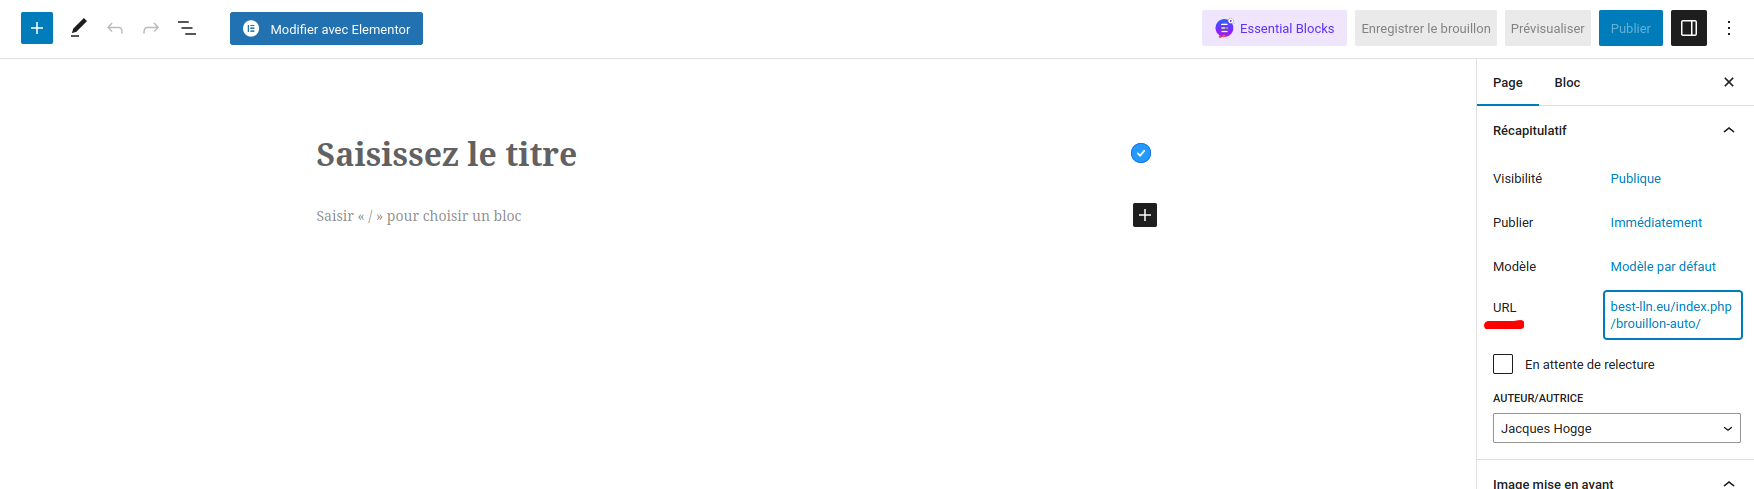
\includegraphics[width=\textwidth]{img/URL.png}
		\end{figure}
		
		Ensuite choisir le modèle sinon le site est trop serrer et moche. Pour cela : Colonne de droite $\rightarrow$ Page $\rightarrow$ Modèle $\rightarrow$  Elementor pleine largeur
		
		\begin{figure}[htp]
			\centering
			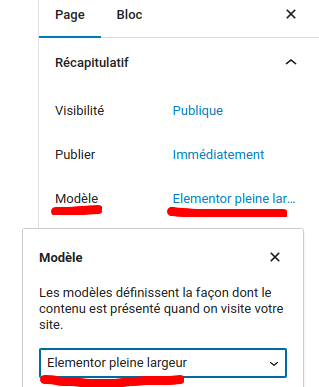
\includegraphics[width=0.3\textwidth]{img/Modele.png}
		\end{figure}
		
		Maintenant on peut commencer a faire notre page. Pour cela, on utilise Elementor qui permet de rendre cela plus intuitif sans trop toucher au HTML et CSS. Si vous voulez un truc bien spécifique il faut coder.
		
		Faite attention de bien suivre le même thème déjà utiliser sur tous le site, venez pas commencer un page avec des coleurs et une structure totalement différente.
		
		\begin{figure}[htp]
			\centering
			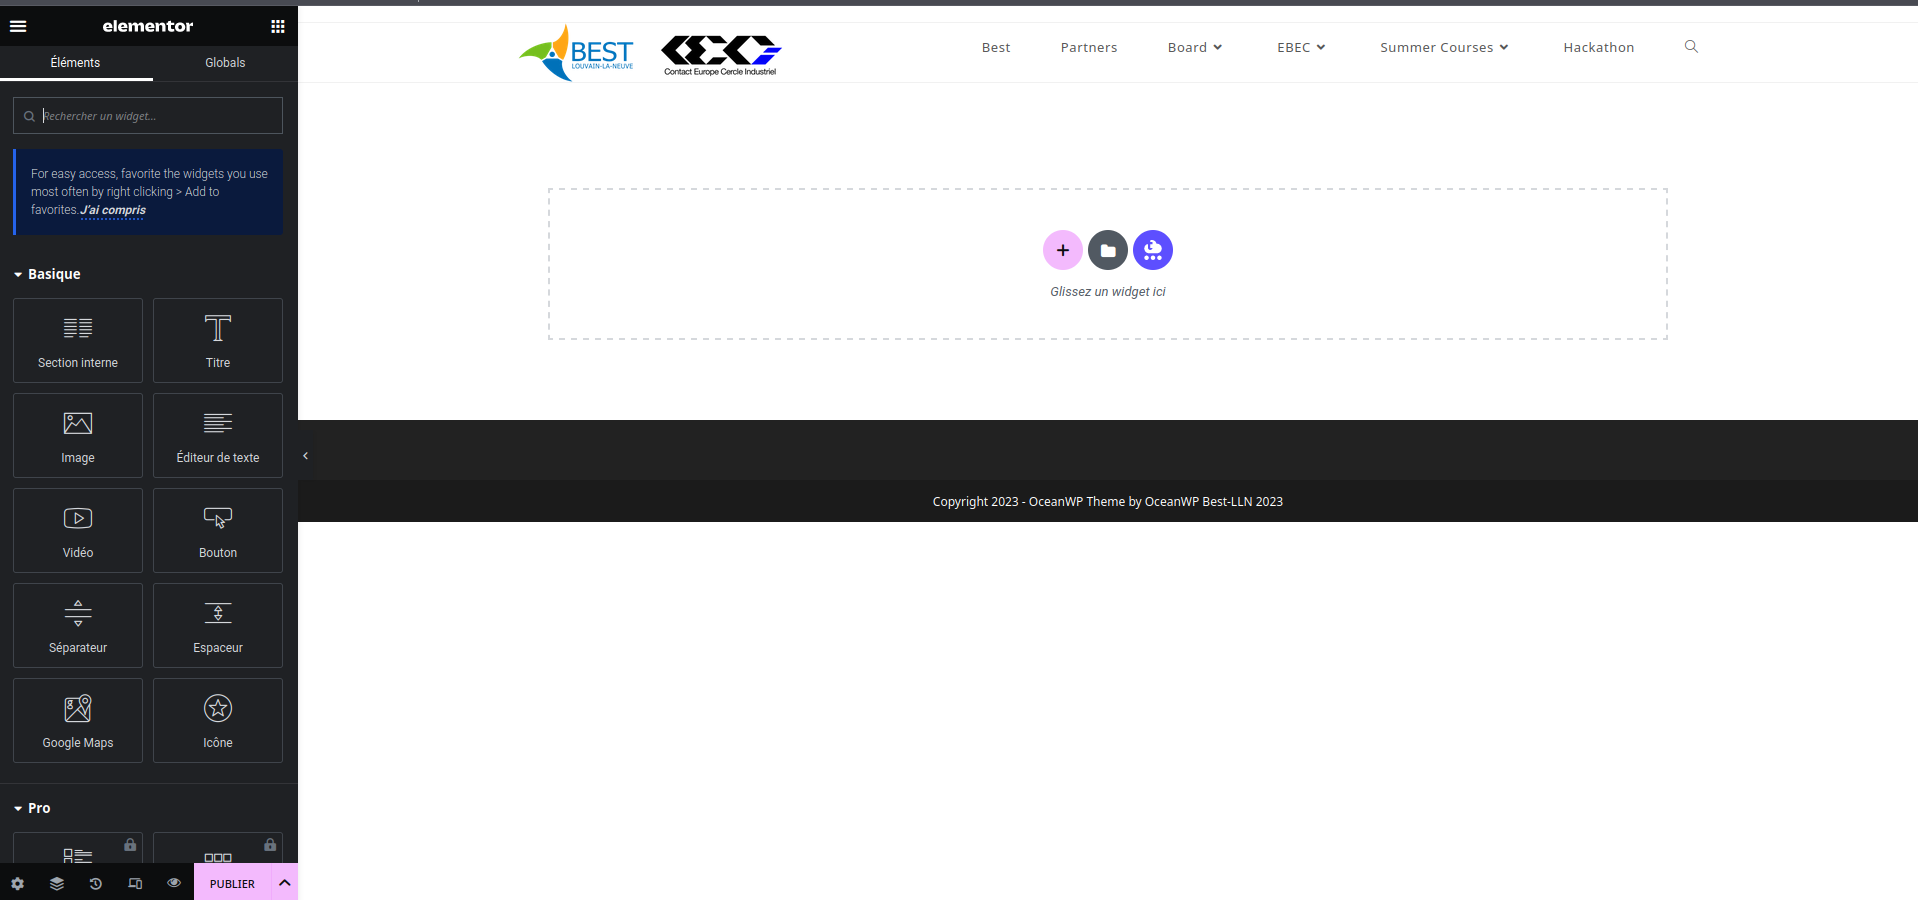
\includegraphics[width=.82\textwidth]{img/PageCreate.png}
		\end{figure}
		
		Attention que ta pages n'est pas accessible tant que tu ne la pas publier avec le boutons en bas a gauche, tu peux meme sauvegarder ta page en brouille pour la modifier plus tard.
		
		Il faut aussi faire attention de rendre la page accessible via le menu. Pour cela rien de dur, il suffit d'aller dans la tableau de bord $\rightarrow$ Apparence $\rightarrow$ Menus
		
		\begin{figure}[htp]
			\centering
			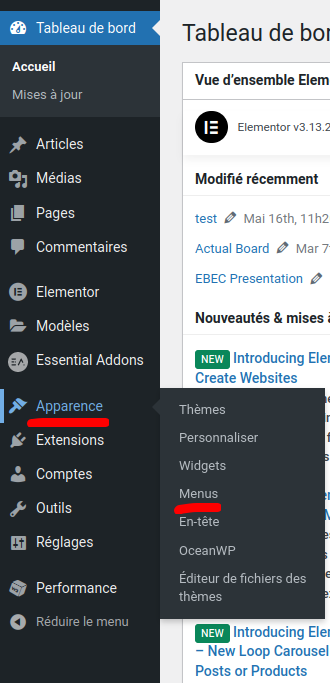
\includegraphics[width=.5\textwidth]{img/Menu.png}
		\end{figure}
		
		Il faut ensuite selectionner votre page dans la partie de gauche et l'ajoute au menu, puis ensuite vous pouvez dans la partie de droite la "Drag and drop" pour la mettre a l'endroit que vous désirer dans le menu.
		
		\begin{figure}[htp]
			\centering
			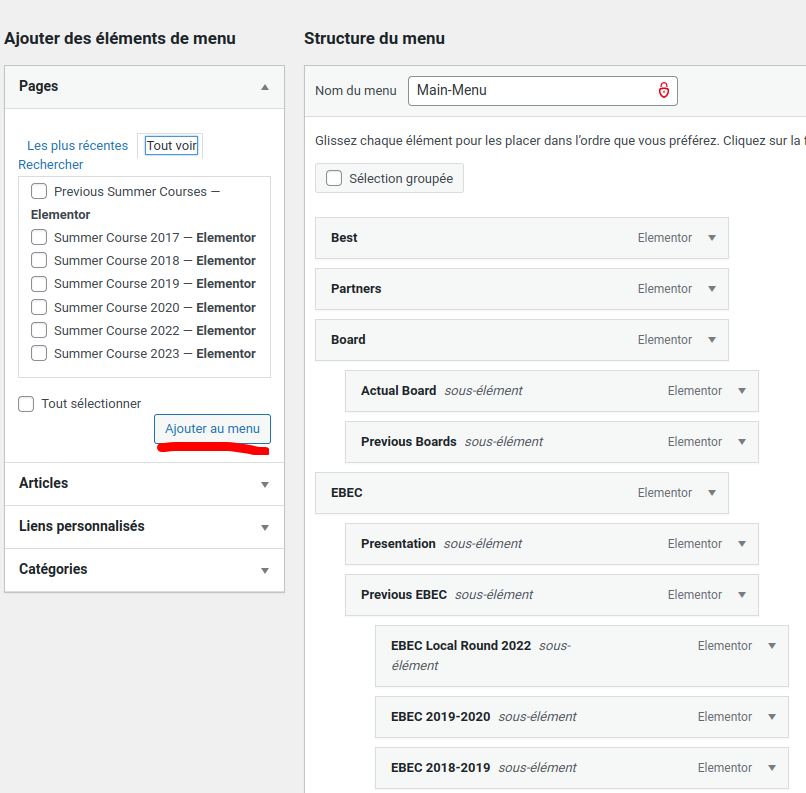
\includegraphics[width=.7\textwidth]{img/Menu1.png}
		\end{figure}
		\vfill
		
		A partir de maintenant c'est toi l'artiste, il y a de nombreux tuto sur youtube si jamais tu as des question et tu peux meme demander a d'ancien IT.
		
	\subsection{Editer une page}
		c'est un peu pareil que pour créer un page mais la il suffit d'aller dans le tableau de bord de Wordpresse $\Rightarrow$ Pages $\Rightarrow$ Toutes les pages.
	
		Tu auras donc la liste de toutes les pages de ton site et tu auras la possiblilité de faire plusieur action dessus tel que les copier, supprimer, modifier ...
		
		\begin{figure}[htp]
			\centering
			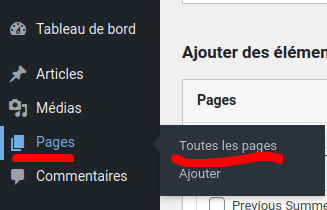
\includegraphics[width=.6\textwidth]{img/EditPage.png}
			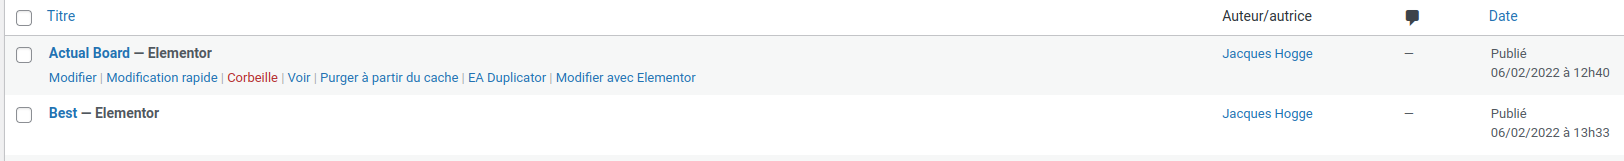
\includegraphics[width=.8\textwidth]{img/EditPage1.png}
		\end{figure}
		
	\subsection{Sponsors}
			
		Il est obligatoire de tenir notre pages des sponsors a jour, c'est dans le contrat que on leur donneras de la visibilité donc si on le fait pas on est dans la merde.
		Pour se faire, il suffit de demander au FR quelle sponsors doivent etres mis sur le site et avec quelle photo et texte. Il ne faut pas hesiter a obliger les photos et le texte au FR car peut etre que les entreprises on des exigences particulière. Ou alors vous pouvez aller voire dans le drive du FR, si celui-ci est doué, tous est la.
	
	Attention certain sponsors sont a l'année alors que d'autre sont peut etre juste pour un événement, a toi de demander et savoir mettre en jour en fonction de cela. 
	
	La page est asser simple a faire, il suffit juste de remprendre l'ancienne et de changer les photo et le texte. Apres libre a toi de tenter de nouvelle choses.
		
	En plus de la page sponsors, il faut aussi les ajouter sur la page  de l'event, soit vous les ajouter comme de simple image qui redirige vers la page sponsors si vous cliquer dessus sois vous faite un "carrousel de photo" qui la aussi si on clique sur un image ramène vers la pages sponsors.
		
		Pour implémenter la redirections, Google et Youtube son votre amis mais avec un peu de chipotage dans le menu vous trouverez assez rapidement.
	
	\subsection{Anciens Board}
		Plus un blague que un point réel mais les anciens veule le moment de gloire et oblige que il soit présent sur la page des anciens Board avec l'année du board et le Nom de celui-ci avec chaque photo et leur poste.
	
	
\section{OVH}
	OVH est notre hebergeur pour le site\footnote{On espère que le serveur ne brulera pas} et qui attribue les domaines \textit{www.best-lln.eu} et \textit{www.best-lln.be}\footnote{C'est le nom de domaine de l'ancien site, on a garder le nom de domaine et fait une redirection vers le nouveau site, ça coute pas trop cher donc a voir avec la trésoreries si vous le laisser ou pas}. 
	\subsection{Creer un sauvegarde}
	\label{creersauvegarde}
		Pour ce faire, il faut se connecter au compte OVH, se rendre sur l'hébergement \textit{best.lln.eu}
		
		\begin{figure}[htp]
			\centering
			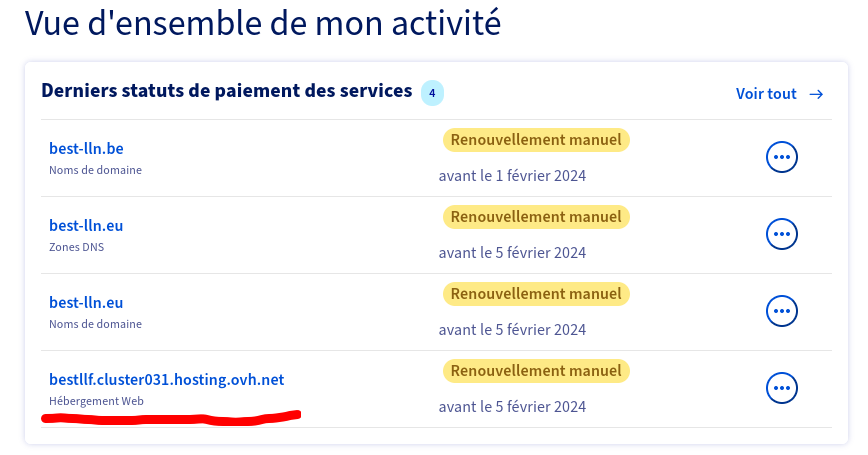
\includegraphics[width=0.5\textwidth]{img/OVH.png}
		\end{figure}
		
		\vfill
		
		\begin{figure}[htp]
			\centering
			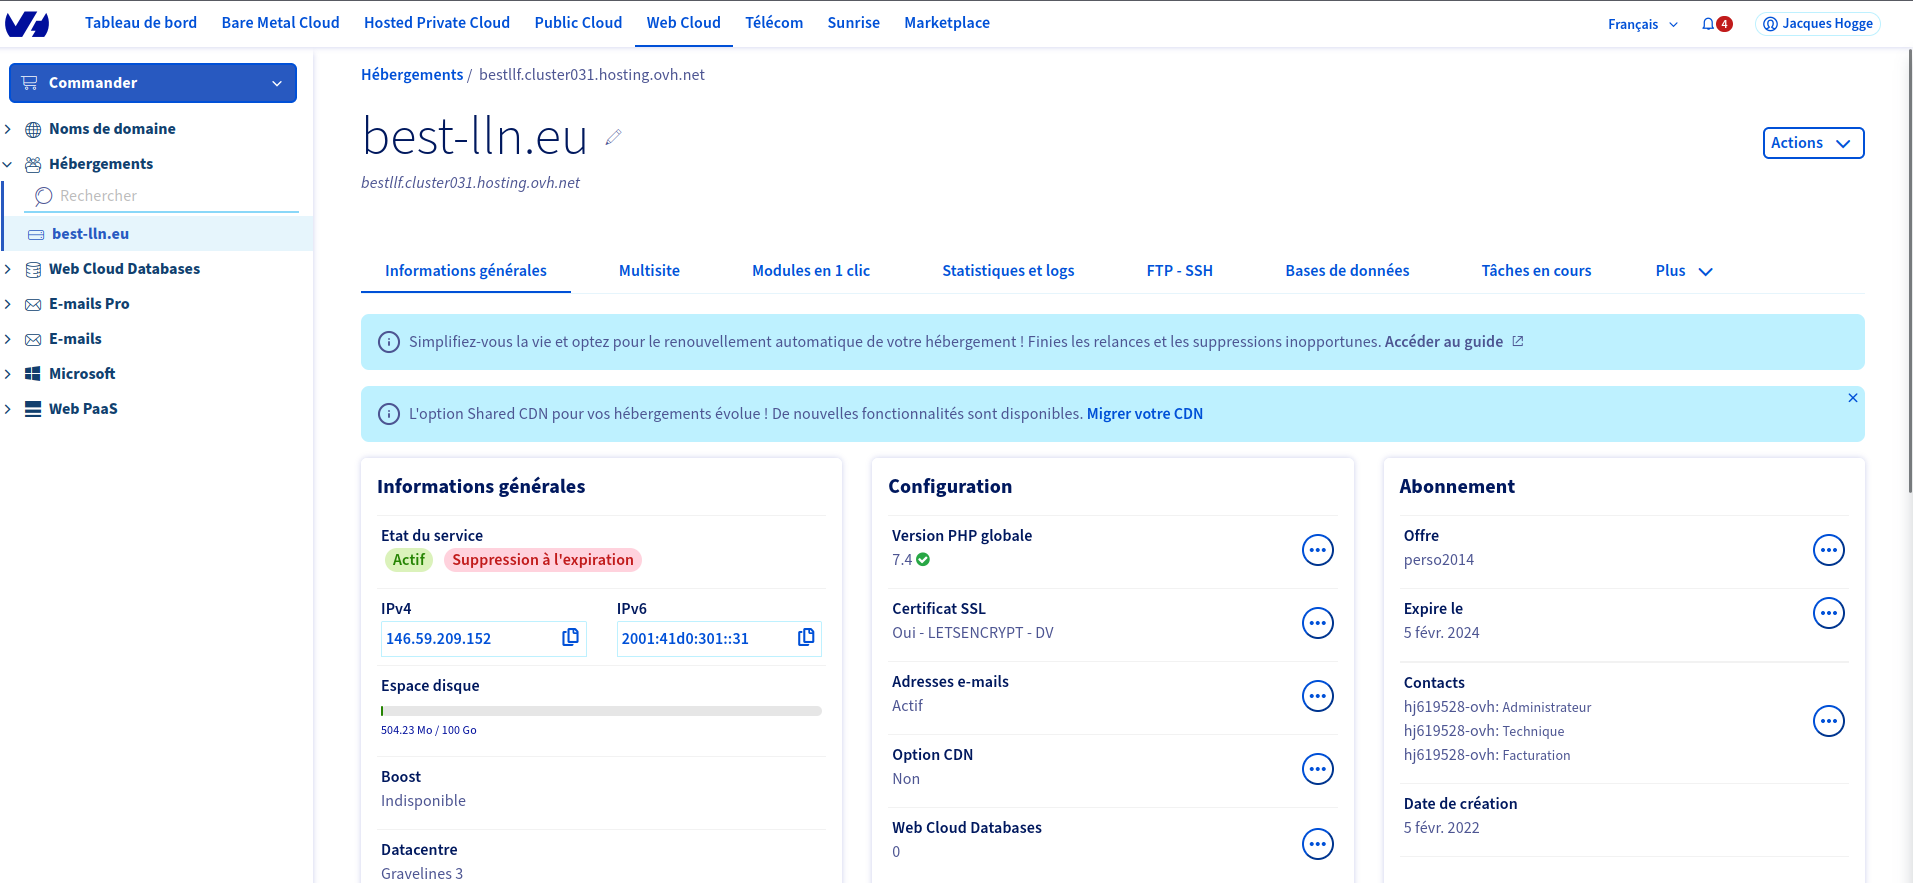
\includegraphics[width=.8\textwidth]{img/OVH1.png}
		\end{figure}
		
		Il y a plein de fonctionnalité que vous pouvez découvrir, ne faite pas trop de betise cela-dit. Pour la sauvegarde, il faut aller dans Bases de données. Une fois la dedans, il suffit de cliquer sur les 3 points et faire "Creer une sauvegarde" et choisir la date d'aujourdhui.
		
		Pour l'instant il y a encore de la place pour pas mal de sauvegarde mais au fil du temps hesiter pas a retirer les trop ancienne. Et si vous vous chauffer vous pouvez mettre les anciennes sauvegarde dans la \textit{Wayback machine}\footnote{\url{https://archive.org/web/}} et ainsi voir dans le futur a quoi ressemblait le site avant.
		
		\begin{figure}[htp]
			\centering
			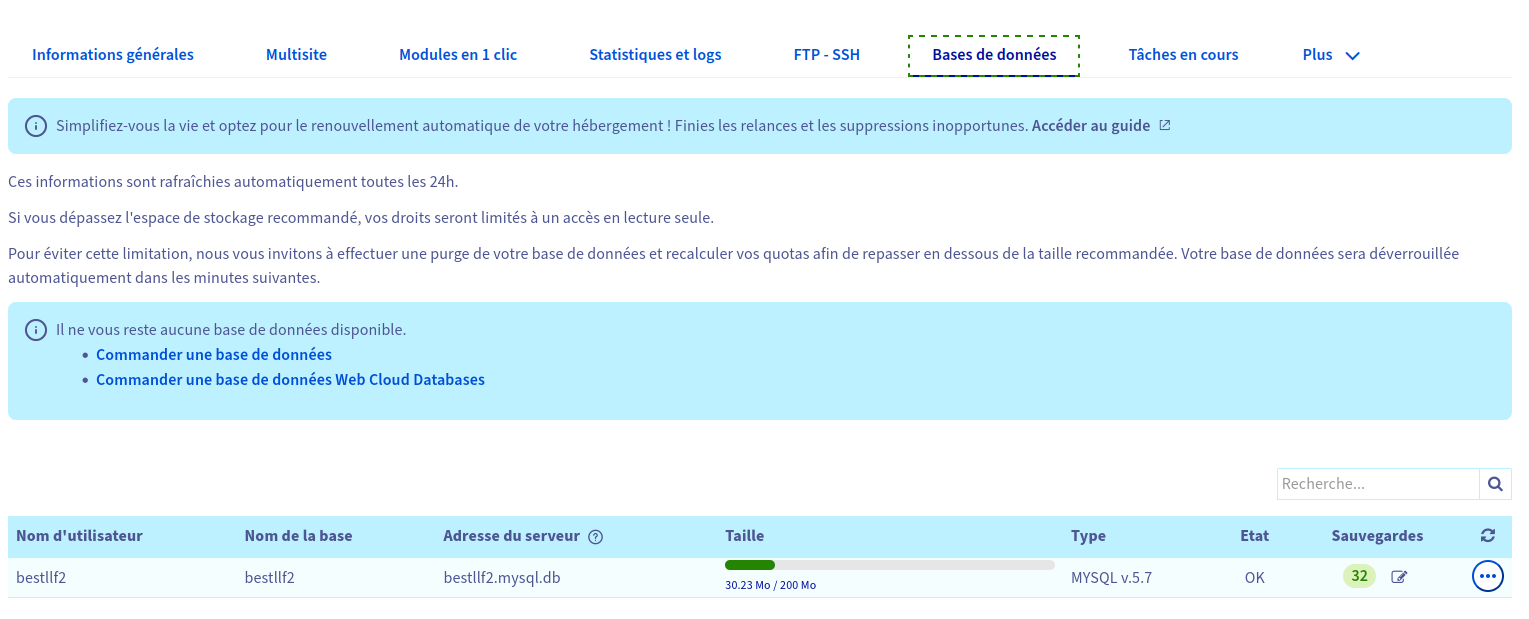
\includegraphics[width=.8\textwidth]{img/OVH2.png}
		\end{figure}
		
	
	\subsection{Récupérer une sauvegarde du site}
		Si jamais tu as fait une connerie, ou que tu veux revenir en arrière, il suffit de faire comment dans la \autoref{creersauvegarde} mais au lieu de créer un nouvelle sauvegarde, il faut \textit{Restaurer une sauvegarde} et voila.
		
	\subsection{Redirection}
		Il y a une redirection qui est faite avec le nom de domaine \textit{www.best-lln.be}. Il suffit d'aller dans le menu a gauche dans Noms de domaine $\rightarrow$ best-lln.be $\rightarrow$ Redirection. et la tu voix toutes les redirection, la plus part sont en lien avec le DNS ou les CNAME donc ne t'en occupe pas. Tu peux en ajouter une nouvelle avec \textit{Ajouter une redirection} a droite.
		
	\subsection{Autre}
		Il y a plein d'autre fonctionnalité sur OVH tels que voire le trafic sur le site etc. Hesite pas a visiter et google les ton amis et les anciens IT aussi
		
\section{Github}
	Depuis 2023 le CECI-BEST possède une github qui est nécessaire pour les Hackhaton qui sont organisé. La responsabilité est techniquement celle de l'IT qui devra aller voire les différent groupes afin de s'ajouter sur le git et garder ainsi une archive. Vous pouvrez aussi les télécharger si vous avez peur que il vont disparetre
	
	les identifiant sont sur le drive et sinon vous pouvez demander a un ancien IT ou a la PR qui normalement doit les connaitres.

	Sur le github, il y a moyen des créer des "dossier" qui comporte different repo github. il suffit d'en créer un par année et de rajouter les repos dedans. Cela est possible avec le syteme "favoris".
	
	Google est ton amis et regarde comment c'est fait avant.
	
\section{Changement proprio Wordpress}
	A faire avec l'ancien IT
	\begin{enumerate}
		\item Ancien IT ajoute le nouveau IT dans les responsable du Wordpress via l’onglet Utilisateurs de l’interface Wordpress

		\item Le nouveau IT donne quand a lui sont adresse mail et sont identifiant
	\end{enumerate}
	

\section{Changement proprio OVH}
	\begin{enumerate}
		\item Le nouvel IT se crée un compte avec son adresse perso (ou BEST comme il veut)
		\item le nouvel IT donne sont identifiant a l'ancien IT (truc du genre aa123456-ovh)
		\item L’ancien gestionnaire change les contacts pour l’hébergement, emails, zone dns et domaine dans son espace OVH (Plus > Gérer les contacts)
		\item Confirmation par mail des 2 coté
	\end{enumerate}
	
\section{Hacked}	
	Il est déja arrivé plusieur fois que on se soit fait Hacker. On parle plus d'un malware qui redirige notre site vers un site de scam. Souvent c'est parceque une script Js a été ajouté dans le header, il font donc le retrouver et le retirer.

Le plus souvent les raisons de ce problèmes  ne sont pas de vous mais de Wordpress et plus particulièrement Elementor qui laisse des breches de sécurité et qui permet au hacker de se connecter au compte. Il faut donc bien faire attention durant les grosse mise-a-jour et voire les différente modification. Et aussi peut etre un peu attendre avant pour voir si il font pas des mise-a-jour de la sécurité juste apres.
	
	Verifier aussi de temps-en-temps si des comptes ne se sont pas rajouter, si c'est le cas, changer tous de suite les mots-de-passe. Ajouter aussi une authentification a double facteur.
	
\section{PHP}
	Notre site est sous PHP avec wordpress, le soucis est que c'est voué a disparaitre, PHP n'est plus aussi sécurisé et utile que avant. Donc petit conseille de ma part. Continuer de garder, et si un jour celui-ci est mort, ne refaite pas un Wordpresse et passer a autre chose. Il est peut etre possible d'utiliser Odoo gratuitement et même avoir un partenaria avec eu justement.



\section{Poste}

	IT est un poste qui selon certaines personnes ne sert a rien ou ne travaille pas. Peut importe ce que tu dit il diront que tu ne fais rien et cela est normal car ce que tu fais n'est pas directement visible
	
	Donc faut pas le prendre mal quand il disent que tu fais riens.
	\subsection{Slides}
	
	l'IT est aussi responsable du rétroprojecteur qui est au local et qu'il faut prendre pour afficher les slides au réunions. rien de tres sorcier il suffit de demander au gens de mettre les slides dans ton fichiers du drives
	
	\subsection{Wooclap}
		Lors de gros vote important (proposale, membership ...) vous utiliserez un wooclap afin d'avoir un systheme de votes pour chaque membre de la réunions. Il suffit de creer un comptes (je conseille d'utiliser l'adresse UCL car tu as le prémium gratuit et donc un nombre illimité de wooclap).
		
	\subsection{Clown}
		L'IT est la personne la plus drole du Board, c'est comme ça c'est la regles, il faut donc tous le temps dires des blagues et faire des bullshit marrant. Attention il faut savoir etre sérieux quand il le faut
	
	\subsection{\textcolor{red}{TRITOUFS}}
		
		La tradition veut que les IT soient des gens expérimentés dans l’art de BWAR. il faut donc se spécialisé dans l’art du Tritouf au fil de mon mandat, c’est pourquoi c’est un plus pour ton poste si tu sais bien en faire (Ca va chier au rachat). 
		
		\begin{enumerate}
			\item Se munir de trois gobelets (réutilisables \#GreenTeam) 
			\item Les remplir généreusement avec de la bière
			\item Les aligner selon ta bonne guise 
			\item Souffler un bon coup 
			\item Boire le premier 
			\item Boire le deuxieme
			\item Boire le troisieme
			\item Éventuellement vomir
			\item Recommencer à partir du point 1. 

		\end{enumerate}
		
		Le but étant bien sûr de vider tous ses verres ENTIÈREMENT. Pas nécessairement le plus vite possible MAIS c’est un plus, naturellement.   


		De nombreuses séances d'apprentissage seront organisées pendant le Summer Course ainsi que des séances d’examen. Bonne chance. 


\section{Conclusion}
	Le post IT c'est le meilleur
		
		
\end{document}